\documentclass[a4paper,12pt,oneside]{mwbk}

%do polskiego wydania
\usepackage[cp1250]{inputenc}
\usepackage{polski}

%do wstawiany obrazk�w
\usepackage{graphicx}

%nag��wki
\pagestyle{uheadings}

%ustawienia storny
\oddsidemargin = 10pt
\textwidth = 470pt

%1,5 linii odst�pu
\linespread{1,3}

%numerowanie definicji
	\newtheorem {definicja}{Definicja}[chapter]%[section]
%numerowanie przyk�ad�w
	\newtheorem {przyklad}{Przyk�ad}[chapter]%[section]

\begin{document}
%spis tre�ci
%			\tableofcontents
%------------------------------------------------------------

%teza, cel i zakres pracy
			\chapter{Wst�p} \label{roz:wstep}
\section{Teza, cel i~zakres pracy}


Punkt wyj�cia, okoliczno�ci powstania problemu, niewystarczalno�� istniej�cych rozwi�za�

Metoda badawcza
\begin{itemize}
\item Studia literaturowe
\item Analiza budowy i dzia�ania istniej�cych produkt�w
\item Projektowanie i prototypowanie nowatorskich rozwi�za� 
\item Obliczenia i ........
\end{itemize}

Co, w kt�rym rozdziale.
%rozdzia� 1
\vspace{12pt} Oto zakres materia�u b�d�cy tre�ci� pracy. Na pocz�tku zawarto przegl�d metod tworz�cych podsumowania dokument�w tekstowych. Spojrzenie na to zagadnienie z~perspektywy kilkunastu ostatnich lat zosta�o opisane w~Rozdziale \ref{roz:wstep}.

%rodzia� 2
Rozdzia� \ref{roz:zbiory} zawiera podstawowe definicje zbior�w i poj�� wykorzystywanych w~rozprawie, takie jak zbiory klasyczne, zbiory rozmyte i~zmienna lingwistyczna oraz ich rozszerzenia ---~intuicjonistyczne zbiory rozmyte i~zbiory rozmyte drugiego rodzaju. 

%rozdzia� 3
Rozdzia� \ref{roz:noweSposobyPodsumowan} zawiera opis podsumowa� Yager'a oraz rozszerzenia tych podsumowa� tj.~podsumowania wieloatrybutowe George'a i~Srikantha oraz wska�niki jako�ci oceniaj�ce poprawno�� podsumowania. Przedstawiono tak�e dalsze prace oparte o~teori� podsumowa� lingwistycznych, w~tym istotne wyniki uzyskane przez Kacprzyka~\cite{KacprzykZadrozny} ---~ \cite{KacprzykZadrozny6}.

%rozdzia� 4
W~Rozdziale \ref{roz:rysunki} znajduj� si� przyk�ady zastosowa� opisanych wcze�niej metod tworzenia podsumowa� lingwistycznych oraz opis systemu komputerowego automatycznie generuj�cego podsumowania wraz z wnioskami wynikaj�cymi z testowania tego systemu.

%reszta rozdzia��w
Kolejne cz�ci to bibliografia, spis rysunk�w i~tabel oraz skorowidz najwa�niejszych poj�� wyst�puj�cych w~rozprawie.
%------------------------------------------------------------

%zbiory klasyczne
%			\chapter{Elementy teorii zbior�w} \label{roz:zbiory}

W~rozdziale przedstawiono podstawowe informacje o~zbiorach w~uj�ciu tradycyjnym np.~\cite{Rasiowa}, o~zbiorach rozmytych np.~\cite{Bandemer, Buckley, Leski, Rutkowscy, Zadeh}. Nie nale�y jednak tego rozdzia�u traktowa� jako kompendium wiedzy, poniewa� znajduj� si� w~nim tylko podstawowe informacje o~zbiorach niezb�dne w~dalszej cz�ci pracy.

\section{Zbiory w uj�ciu klasycznym}

%definicja zbioru
\begin{definicja}
	Przez zbi�r rozumie si� grup� obiekt�w o~pewnych w�asno�ciach wyr�niaj�cych je spo�r�d innych obiekt�w. 
	Obiekty z~tej grupy s� elementami zbioru, a~zatem musz� spe�nia� pewn� w�asno�� charakterystyczn� dla danego 
	zbioru:
	\begin{equation}
		Z = \{x \in X:\mu_C(x)\}
	\end{equation}
	gdzie:\\
	\indent	$X = \{x\}$ jest zbiorem wszystkich mo�liwych obiekt�w, zwanych przestrzeni�,\\
	\indent $\mu_C(x)$ jest funkcj� charakterystyczn�, okre�laj�c� przynale�no�� do zbioru, tzn.
	\begin{equation}
		\mu_C(x)=
			\left\{
				\begin{array}{ll}
					1, & \mbox{gdy $x \in Z$} \\
					0, & \mbox{gdy $x \not\in Z$}
				\end{array}
			\right.
	\end{equation}
\end{definicja}

%przyk�ad zbioru
\begin{przyklad}
	Dany jest zbi�r $A$ okre�laj�cy wielko�� firmy na podstawie liczby zatrudnionych pracownik�w. Rozpatrzmy przynale�no�� do zbioru {\em mikro}-firma, dla kt�rej funkcja charakterystyczna ma posta�\footnote{wielko�ci zdefiniowane na podstawie rozporz�dze� Unii Europejskiej}: 
	\begin{displaymath}
		\mu_A(x)=
			\left\{
				\begin{array}{ll}
					1, & \mbox{gdy $5 < x < 15$} \\
					0, & \mbox{gdy le�y poza powy�szym przedzia�em}
				\end{array}
			\right..
	\end{displaymath}
Zatem firma maj�ca wi�cej ni� $5$ i~mniej ni� $15$ pracownik�w nale�y do grupy firm typu {\em mikro} poniewa� $\mu_A(5-15)=1$, natomiast dla firm o~liczbie pracownik�w mniejszej ni� $5$ i wi�kszej ni� $15$ pracownik�w przynale�no�� do zbioru wynosi~$0$ (bo $\mu_A(<5 \ i \ >15)=0$), zatem ta ta firma nie nale�y do zbioru {\em mikro}.
\end{przyklad}

%definicja zawierania zbior�w
\begin{definicja}
	Zbi�r $A$ jest zawarty w~zbiorze $B$ ($A \subset B$) wtedy i~tylko wtedy, gdy ka�dy element zbioru $A$ jest elementem zbioru $B$, co zapisujemy:
	\begin{equation}
		A \subset B \Leftrightarrow \{x: x \in A \Rightarrow x \in B\}
	\end{equation}
\end{definicja}

%defincja r�wno�ci zbior�w
\begin{definicja}
	Zbiory $A$ i~$B$ s� r�wne, gdy ka�dy element zbioru $A$ jest elementem zbioru~$B$.
	\begin{equation}
		\forall_x (x \in A \Leftrightarrow x \in B)
	\end{equation}
\end{definicja}

%definicja sumy zbior�w
\begin{definicja}
	Przez sum� zbior�w $A$ i~$B$ (oznaczmy j� $A \cup B$) rozumiemy zbi�r, kt�rego elementami s� wszystkie 
	elementy zbioru $A$ i~wszystkie elementy zbioru $B$, ponadto zbi�r ten nie zawiera innych element�w, czyli:
	\begin{equation}
		A \cup B = \{x: x \in A \vee x \in B\}
	\end{equation}
	Inaczej mo�na to zapisa�, �e:
	\begin{equation}
		(A \cup B)(x) = max \{\mu_A(x), \mu_B(x)\}	
	\end{equation}
\end{definicja}

%definicja iloczynu zbior�w
\begin{definicja}
	Przez iloczyn zbior�w $A$ i~$B$ (oznaczmy go $A \cap B$) rozumiemy cz�� wsp�ln� zbior�w, czyli zbi�r
	zawieraj�cy te i~tylko te elementy, kt�re nale�� jednocze�nie do zbioru $A$	i~zbioru $B$, czyli:
	\begin{equation} 			
		A \cap B = \{x: x \in A \wedge x \in B\}
	\end{equation}
	lub:
	\begin{equation}
		(A \cap B)(x) = min \{\mu_A(x), \mu_B(x)\}
	\end{equation}
\end{definicja}

%przyk�ad na sum� i iloczyn zbior�w
\begin{przyklad}	\label{przyk:sumaIloczyn}
	Dany jest zbi�r $A$ okre�laj�cy wielko�� {\em mikro}-firmy na podstawie liczby zatrudnionych pracownik�w
	\begin{displaymath}
		\mu_A(x)=
			\left\{
					\begin{array}{ll}
					1, & \mbox{gdy $5 < x \leq 15$} \\
					0, & \mbox{gdy le�y poza powy�szym przedzia�em}
				\end{array}
			\right.
	\end{displaymath}
  oraz zbi�r $B$ definiuj�cy {\em �rednie}-firmy r�wnie� na podstawie liczby zatrudnionych pracownik�w
	\begin{displaymath}
		\mu_B(x)=
			\left\{
				\begin{array}{ll}
					1, & \mbox{gdy $14 < x < 50$} \\
					0, & \mbox{gdy le�y poza powy�szym przedzia�em}
				\end{array}
			\right.
	.\end{displaymath}
	Sum� zbior�w $A$ i $B$ jest zbi�r $C$, do kt�rego nale�� {\em mikro} i~{\em �rednie} firmy, dla kt�rych 
	liczba zatrudnionych pracownik�w jest z~przedzia�u~$[5-50]$, poniewa�
	\begin{displaymath}
		\mu_{A \cup B}(x)=
			\left\{
				\begin{array}{ll}
					1, & \mbox{gdy $5 < x < 50$} \\
					0, & \mbox{gdy le�y poza powy�szym przedzia�em}
				\end{array}
			\right.
	.\end{displaymath}
	Natomiast iloczyn tych dw�ch zbior�w to firmy zatrudniaj�ce dok�adnie $15$ pracownik�w, poniewa� 
	\begin{displaymath}
		\mu_{A \cap B}(x)=
			\left\{
				\begin{array}{ll}
					1, & \mbox{gdy $x = 15$} \\
					0, & \mbox{gdy le�y poza powy�szym przedzia�em}
				\end{array}
			\right.
	.\end{displaymath}
\end{przyklad}

%definicja dope�nienia
\begin{definicja}
	Dope�nieniem zbioru $A$ (oznaczamy je $\neg A$) w~przestrzeni $X$ ($A \subset X$) nazywamy zbi�r wszystkich 
	element�w, kt�re nie nale�� do zbioru $A$, czyli:
	\begin{equation}
		\neg A = \{x: x \in X \wedge x \not \in A\}
	\end{equation}
	Stosuj�c zapis dla funkcji charakterystycznych dope�nienie zbioru $A$ mo�na zapisa� jako:
	\begin{equation}
		\mu_{\neg A} = 1 - \mu_A(x)
	\end{equation}
\end{definicja}

%przyk�ad dope�nienia
\begin{przyklad}
	Dany jest zbi�r $A$ {\em mikro}-firm, dla kt�rego funkcja charakterystyczna ma posta� jak w~Przyk�adzie \ref{przyk:sumaIloczyn}. Dope�nieniem tego zbioru b�d� firmy nie nale��ce do tego zbioru, a~zatem firmy zatrudniaj�ce wi�cej ni� $15$ i~mniej ni� $5$ pracownik�w.
\end{przyklad}

%definicja pary uporz�dkowanej
\begin{definicja}
	Zbi�r postaci $\{a, b\}$ nazywamy uporz�dkowan� par� element�w $a$ i~$b$.
\end{definicja}

%definicja iloczynu kartezja�skiego
\begin{definicja}
	Niech dane b�d� dwa zbiory $A$ i~$B$. Zbi�r z�o�ony ze wszystkich par uporz�dkowanych postaci $<a, b>$ takich, �e $a \in A$ i $b \in B$ nazywamy iloczynem kartezja�skim zbior�w $A$ i~$B$ i~oznaczamy $A \times B$.
\end{definicja}
\vspace{6pt}
%w�asno�ci na zbiorach
{\bf Podstawowe w�asno�ci zbior�w klasycznych:}
%\newline W�asno�� przemienno�ci zdefiniowana nast�puj�co:  \index{zbi�r!klasyczny!przemienno��}
\begin{itemize}
	\item W�asno�� przemienno�ci zdefiniowana nast�puj�co:  \index{zbi�r!klasyczny!przemienno��}
			\begin{equation} \label{wzor:przemiennoscZbiorKlasyczny}
				\begin{array}{c}
					A \cup B = B \cup A\\
					A \cap B = B \cap A
				\end{array}
			\end{equation}
		U�ywaj�c funkcji charakterystycznych powy�sz� w�asno�� mo�na zapisa� nast�puj�co:
			\begin{equation}
				(A \cup \neg A)(x) = max \{\mu_A(x), 1-\mu_A\} = 1
			\end{equation} 	
	\item Prawo ��czno�ci: \index{zbi�r!klasyczny!��czno��}
			\begin{equation} 	\label{wzor:lacznoscZbiorKlasyczny}
					(A \cup B) \cup C = A \cup (B \cup C)
			\end{equation}
	\item Prawo rozdzielno�ci: \index{zbi�r!klasyczny!rozdzielno��}
			\begin{equation} \label{wzor:rozdzielonoscZbiorKlasyczny}
				(A \cup B) \cap C = (A \cap C) \cup (B \cap C)
			\end{equation}
	\item Prawo dope�nienia: \index{zbi�r!klasyczny!dope�nienie}
			\begin{equation}
				\begin{array}{c}
					A \cup \neg A = X \\
					A \cap \neg A = \oslash 
				\end{array}
			\end{equation}
		Zapis przy u�yciu funkcji charakterystycznych:
			\begin{equation}
				(A \cap -A)(x) = min \{\mu_A(x), 1 - \mu_A(x)\} = 0
			\end{equation}
\end{itemize}

%definicja relacji
\begin{definicja}
	Relacj� $\varsigma$ ze zbioru $A$ w~zbi�r $B$ nazywamy podzbi�r b�d�cy iloczynem kartezja�skim $A \times B$.
	Je�eli $<a, b> \in \varsigma$, to m�wimy, �e $a$ jest w~relacji $\varsigma$ z~elementem $b$, co zapisujemy 
	$a \varsigma b$.
\end{definicja}



%podsumowania
		\chapter{Nowe sposoby generowania podsumowa� lingwistycznych} \label{roz:noweSposobyPodsumowan}

Rozw�j technologii komputerowych, a~tak�e sposobu i~ilo�ci zapisywanych danych wymusi� nowe podej�cie do generowania podsumowa� lingwistycznych. Obecnie w~bazach danych przechowywane s� przer�ne informacje zawieraj�ce dane w~postaci numerycznej i~tekstowej. Du�a ilo�� tych ostatnich zapisywana jest w~postaci zda�, wyra�e�, czy te� r�nej wielko�ci plik�w tekstowych. Dotychczasowy spos�b tworzenia podsumowa� nie jest w~stanie zapewni� uniwersalno�ci w~przypadku tak r�norodnych sposob�w reprezentacji danych w~bazie. Kolejne podej�cia do generowania podsumowa� radz� sobie z~informacjami w~postaci tekstowej (szukane jest bowiem podobie�stwo do wzorca podsumowania), jak r�wnie� z~danymi znajduj�cymi si� w~plikach tekstowych~\cite{Ochelska2001}.

Generowanie podsumowa� lingwistycznych nadal opiera si� na koncepcji, kt�r� zaproponowa� Yager~\cite{YagerPodsumowania1, YagerPodsumowania2, YagerPodsumowania3, YagerPodsumowania4}, czyli b�d� to zdania oznajmuj�ce sk�adaj�ce si� z~nast�puj�cych okre�le�:
\begin{itemize}
	\item okre�lenia liczno�ci $Q$,
	\item przedmiotu podsumowania $P$,
	\item interesuj�cej cechy $S$,
	\item wska�nika jako�ci podsumowania $T$.
\end{itemize}

Przedstawiona tu metoda generowania podsumowania jest rozwini�ciem idei Yager'a. Pozwala ona wykona� podsumowanie na r�nych typach danych. Dobrze radzi sobie z~danymi przedstawionymi w~tradycyjnej numerycznej formie oraz z~opisami przedstawionymi w~j�zyku naturalnym (zdania znajduj�ce si� w~bazie, czy te� umieszczone w~plikach tekstowych). Zatem u�ytkownik bazy ma mo�liwo�� otrzymania odpowiedzi na dowolne pytanie dobrze okre�lone w sensie istniej�cej bazy, w~rodzaju ,,{\em Ilu} pacjent�w zosta�o przyj�tych {\em w~wieku �rednim}?'' lub ,,{\em Ilu} pacjent�w zosta�o przyj�tych w~stanie og�lnym {\em dobrym}?''. Odpowiedzi na te pytania s� automatycznie generowane na podstawie podsumowa� lingwistycznych, zatem odpowiedzi� jest r�wnie� zdanie w j�zyku naturalnym zawieraj�ce okre�lenie liczno�ci przedstawione przy u�yciu odpowiedniego zbioru rozmytego. Przyk�adowe podsumowania mog�yby mie� posta�: ,,{\em Wi�kszo��} pacjent�w zosta�a przyj�ta {\em w~wieku �rednim}.'' lub ,,{\em Niewielu} pacjent�w zosta�a przyj�ta w~stanie og�lnym {\em dobrym}.''.

Kolejne podrozdzia�y, to propozycje wykorzystania r�nych mechanizm�w do tworzenia podsumowa�. W~pierwszym opisano generowanie podsumowa� na dokumentach tekstowych (jest to nowy element w~podsumowaniach). W~kolejnym ---~om�wiono mo�liwo�� podsumowywania dokument�w mieszanych (zar�wno danych numerycznych, jak i~wyra�onych w~j�zyku naturalnym). W~celu zmniejszenia niepewno�ci wynikaj�cej z~por�wnywania tekst�w wprowadzono dodatkow� ilo�ciow� miar�, kt�ra ocenia niepodobie�stwo por�wnywanych wyra�e�. Nast�pnie pokazano dwa nowe sposoby wyboru rekord�w do generowania podsumowa�: na podstawie selekcji ostrej i~wnioskowania rozmytego. Ostatni z~podrozdzia��w przedstawia podsumowania z~u�yciem zbior�w rozmytych drugiego rodzaju.

Do ilustracji (Tabela~\ref{tab:BazaPacjentow}) tych zagadnie� wybrano przejrzysty przyk�adowy zbi�r rekord�w, na kt�rym b�d� generowane podsumowania.
\begin{table}[ht]
	\centering
			\begin{tabular}{|c|c|l|}
				\hline
						Lp.	& Wiek pacjenta	& Stan pacjenta podczas przyj�cia do szpitala \\ \hline
						1. & 20 & Stan pacjenta do�� dobry. \\ \hline
						2. & 16 & Pacjent w stanie og�lnym dobrym. \\ \hline
						3. & 73	& Stan og�lny dobry. \\ \hline
						4. & 59	& Stan og�lny pacjenta dobry.\\ \hline
						5. & 19	& Pacjent w stanie og�lnym dobrym.\\ \hline
						6. & 23	& Pacjent w stanie og�lnym dobrym.\\ \hline
						7. & 12	& Pacjentka w stanie og�lnym dobrym.\\ \hline
						8. & 27	& Pacjent w stanie og�lnym bardzo dobrym.\\ \hline
						9. & 26	& Stan og�lny pacjenta bardzo ci�ki.\\ \hline
						10. & 65 & Pacjentka w stanie og�lnym �rednio dobrym. \\ \hline
		\end{tabular}
	\caption{Przyk�adowa baza danych pacjent�w}
	\label{tab:BazaPacjentow}
\end{table}
		
%rysunki
		\chapter{Implementacja} \label{roz:rysunki}

System napisany jest w~j�zyku Java z~wykorzystaniem pakietu~\textsf{java.swing.*}, a zatem jest on niezale�ny od platformy, na kt�rej zostanie uruchomiony. Program, kt�ry wspomaga uruchomienie i~obs�ug� tego programu to Eclipse ---~jest to platforma, kt�ra jest �rodowiskiem s�u��cym do projektowania aplikacji, jak r�wnie� umo�liwiaj�cym tworzenie w�asnych narz�dzi. 
\newline W oparciu o poprzednie podrozdzia�y mo�na wnioskowa�, �e system sk�ada si� z trzech warstw: warstwy danych (bazy danych), warstwy biznesowej (umo�liwiaj�cej przetwarzanie danych) oraz warstwy prezentacji (s�u��cej do komunikacji z~u�ytkownikiem). System ten sk�ada si� zatem z~klas, kt�re odpowiadaj� za poszczeg�lne zadania systemu ---~pobierania danych od u�ytkownika lub z~bazy, ich przetwarzania oraz wysy�ania danych na ekran. Poni�ej zostanie przedstawiony opis systemu z~wykorzystaniem notacji UML\footnote{UML ---~Unified Modeling Language, to graficzny j�zyk do obrazowania, specyfikowania, tworzenia i~dokumentowania element�w system�w informatycznych \cite{UML}.}.

%rysunek - pakiety
\begin{figure}[ht]
	\begin{center}
		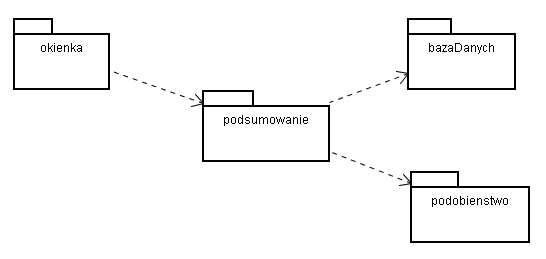
\includegraphics[width=300pt]{UMLPakiety}
		\caption{Pakiety systemu} \label{rys:UMLPakiety}
	\end{center}
\end{figure}

System podzielony jest na pakiety (co wida� na rysunku \ref{rys:UMLPakiety}), kt�re grupuj� klasy odpowiedzialne za dzia�anie systemu. Klasy z~danych pakiet�w komunikuj� si� ze sob� w~celu wymiany danych potrzebnych do wygenerowania podsumowania lingwistycznego. W~pakiecie \textsf{okienka} znajduj� si� wszystkie klasy odpowiedzialne za komunikacj� pomi�dzy u�ytkownikiem, a~systemem (dok�adny opis klas znajduje si� poni�ej). Klasy z~tego pakietu odwo�uj� si� do klas z~pakietu \textsf{podsumowanie}, kt�re po otrzymaniu odpowiednich danych pobranych z~bazy (poprzez klasy z~pakietu \textsf{bazaDanych} i~po przetworzeniu ich przez metody umieszczone w~klasach z~pakietu \textsf{podobienstwo} tworz� podsumowanie lingwistyczne wraz z~warto�ciami poprawno�ci podsumowania. Takie podsumowanie jest nast�pnie wy�wietlane u�ytkownikowi ponownie poprzez klasy z~pakietu~\textsf{okienka}.

%Sprawdzi� poprawno�� i kolejno�� element�w w literaturze

\begin{thebibliography}{100}

	\bibitem{Bandemer} Bandemer H., Gottwald S., {\em	Fuzzy Sets, Fuzzy Logic, Fuzzy Methods with Applications}, 	
		John Willey and Sons, England, 1995.

	\bibitem{UML} Booch G., Rumbaugh J., Jacobson I., {\em UML prze\-wo\-dnik u\-�yt\-kow\-ni\-ka}, Wydawnictwo 
		Nau\-ko\-wo\--Tech\-ni\-czne, Warszawa.

	\bibitem{Buckley} Buckley J.J., Eslami E., {\em An Introduction to Fuzzy Logic and Fuzzy 
		Sets}, Physica-Verlag, Heidedlberg, 2002.
		
	\bibitem{KacprzykZadrozny} Kacprzyk J., Zadrozny S., {\em On Linguistic Approaches in Flexible Querying and Mining of Association Rules}, In. Larsen H.L., Kacprzyk J., Zadro�ny S., Andreasen T., Christiansen H., {\em Flexible Query Answering Systems}, Physica Varlag, Heidelberg, 475-484, 2001.
	\bibitem{KacprzykZadrozny1} Kacprzyk J., Zadrozny S., {\em Computing with words in intelligent database querying:standalone and Internet-based applications}, Information Sciences, 34, 71-109, 2001.
	\bibitem{KacprzykZadrozny2} Kacprzyk J., Zadro�ny S., {\em Fuzzy querying for Microsoft Access}, In. Proceedings of the Third IEEE Conference on Fuzzy Systems, Orlando, USA, col. 1, 167-171, 1999.
	\bibitem{KacprzykZadrozny3} Kacprzyk J., Zadro�ny S., {\em Fuzzy queries in Mocrosoft Access: towards a 'more intelligent' use of Microsoft Windows based DBMSs}, In. Proceedings of the Second Australian and New Zealand Conference on Intelligent Information Systems-ANZIIS'94, Brisbane, Australia, 492-496, 1994.
	\bibitem{KacprzykZadrozny4} Kacprzyk J., Zadro�ny S., {\em FQUERY for Access: fuzzy querying for a Windows-based DBMS}, In. Bosc P., Kacprzyk J., {\em Fuzziness in Database Management System}, Physica-Verlag, Heidelberg, 415-433, 1995.
	\bibitem{KacprzykZadrozny5} Kacprzyk J., Zadro�ny S., {\em Flexible querying using fuzzy logic: An implementation for Microsoft Access}, In. Andreasen T., Christiansen H., Larsen H.L., {\em Flexible Query Answering System}, Kluwer Academic Publishers, Boston, 247-275, 1997.
	\bibitem{KacprzykZadrozny6} Kacprzyk J., Zadro�ny S., {\em Implementation of OWA operators in fuzzy querying for Microsoft Access}, In. Yager R.R., Kacprzyk J., {\em The Ordered Weighted Averaging Operators: Theory and Applications}, Kluwer Academic Publishers, Boston, 293-306, 1997.

	\bibitem{Leski} ��ski J., Straszecka E., {\em	Zbiory rozmyte i ich zastosowanie w diagnostyce medycznej},	In. 
		Zajdel R., K�cki E., Szczepaniak P., Kurzy�ski (red.), {\em Kompendium informatyki medycznej}, 
		Medica-press, Bielsko-Bia�a, 2003.

	\bibitem{Ochelska2001} Ochelska J., Niewiadomski A., Szczepaniak P. S., {\em Linguistic Summaries 
		Applied To Medical Textual Databases}, Dept. of Electronics \& Computer Systems University 	
		of Silesia, Ustro�, 2001.
	\bibitem{Ochelska2004} Ochelska J., Szczepaniak P., Niewiadomski A.,	{\em Automatic Summarization on 
		Standarized Textual Databases Interpreted in Terms of Intuitionistic Fuzzy Sets}, W: Soft Computing Tools, 
		Techniques and Applications, Akademicka Oficyna Wydawnicza EXIT, Warszawa, 2004.
	\bibitem{Ochelska2005} Ochelska J., Szczepaniak P.S., {\em Textual Fuzzy Similarity and Sequence Kernels}, XIII KOnferencja Sieci i Systemy Informatyczne, ��d�, 299-304, 2005.

	\bibitem{Rasiowa} Rasiowa H.,	{\em Wst�p do matematyki wsp�czesnej}, 
		Wydawnictwo Naukowe PWN, Warszawa, 1998.
		
	\bibitem{Rutkowscy} Rutkowska D., Pili�ski M., Rutkowski L., {\em Sieci neuronowe, 
		algorytmy genetyczne i systemy rozmyte}, Wydawnictwo Naukowe PWN, Warszawa-��d�, 1997.

	\bibitem{YagerPodsumowania1} Yager R. R., T. C. Rubinson, {\em Linguistic Summaries of Data 
		Bases}, Proc. IEEE Conference on Decision and Control, San Diego, 1981.
	\bibitem{YagerPodsumowania2} Yager R. R., KFord. M., Canas A. J, {\em On Linguistic Summaries 
		of Data, w Information Processing and Management of Uncertainty in Knowledge-Based System}, 
		3rd International Conference, Paris, France, 1990. 
	\bibitem{YagerPodsumowania4} Yager R. R., {\em On Linguistic Summaries of Data}, w Knowledge 
	  Discovery in Databases, Piatetsky-Shapiro, G. \& Frawley, B. (eds.), Cambridge, 1991.
	\bibitem{YagerPodsumowania3}	Yager R. R., {\em Linguistic summaries as a tool for database 
		discovery}, Workshop on Fuzzy Database System and Information Retrival, Yokohama, 
		Japan 1995. 

	\bibitem{Zadeh} Zadeh L.A., {\em Fuzzy Sets}, Information and Control 8, 1965.
\end{thebibliography}

%------------------------------------------------------------
%spis rysunk�w
		\listoffigures
%------------------------------------------------------------
%spis tabel
			\listoftables
%------------------------------------------------------------
\end{document}